% *- coding: UTF-8 -*-
% !TEX builder = Texlive
% !TEX prggram = xelatex
\documentclass[UTF8,a4paper,12pt,titlepage]{ctexart}
% tittlepage制作一个封面
% draft是草稿,有个方框
%\documentclass[UTF8,a4paper,11pt]{book}

%\CTEXsetup[name={第,章}]{section}%每section统一名称

%每章节题目统一格式
\CTEXsetup[format={\zihao{-3}\raggedright\bfseries}]
{section}

\newcommand{\keyword}[1]{\textbf{#1}}

%\usepackage{microtype}

% 纸张格式
\usepackage[paper=a4paper,inner=1.5cm,outer=2cm,top=2cm,
bottom=2.5cm,bindingoffset=0.5cm]{geometry}

\usepackage[onehalfspacing]{setspace} % 1.5倍行距

% 自动链接内容
\usepackage[colorlinks=true,linkcolor=black]{hyperref}
% 设置文件属性内容
\hypersetup{pdfauthor={吴毓明},
            pdftitle={高锰酸钾制备自动投加装置},
            pdfsubject={使用说明},
            pdfkeywords={任何问题,联系61508712@qq.com}}

% 定义页眉页脚
% 定义页眉页脚
\usepackage{fancyhdr}
\fancyhf{}
\pagestyle{fancy}
% 公共
\rhead{\zihao{6}一体化全自动加药装置/化工泵\\
       Manage Pump as Diamond} % 页眉右

% 利亨昌
% \lhead{
\includegraphics{LHC-head.png}}% 页眉左
% \lhead{
\includegraphics[height=0.5cm]{LHC.jpg}} % 页眉左
% \chead{\zihao{4}广州市利亨昌贸易有限公司}
% \chead{\zihao{5}广州市利亨昌贸易有限公司}
% \lfoot{\zihao{6}广州市荔湾区东联路2号工业园\\
%                电话:020-8430 1397 传真:020-84301170 \\ 
%                电邮:gzlhcmy@163.com 网址:www.lhcmy.com}
% \cfoot{\thepage} % 页脚右
% \cfoot{\zihao{5}\thepage} % 页脚中
% \rfoot{\zihao{6}美国帕斯菲达PULSAFEEDER 产品库存商\\Paddle-flow流量监控及加药装置} % 页脚右
% \rfoot{\zihao{6}美国帕斯菲达PULSAFEEDER 产品库存商\\Paddle-flow流量监控及加药装置} % 页脚右
% \rfoot{\thepage} % 页脚右

% paddle-flow
%\rhead{\includegraphics{paddle-flow.png}}

% 厦门飞华
\lfoot{厦门飞华环保有限公司}
\rfoot{\thepage} % 页脚右



\renewcommand{\headrulewidth}{0.4pt} % 页眉分隔线
\renewcommand{\footrulewidth}{0.4pt} % 页脚分隔线

% 表格 定义表头字体
\newcommand{\head}[1]{\textnormal{\textbf{#1}}}

% 表格 特殊命令,见后文 array
% 在竖向多种对齐方式
\usepackage{array}
\setlength{\extrarowheight}{4pt} % 增加列距
\usepackage{booktabs} % 用于美化表格的线
\usepackage{multirow} % 合并行
\newcommand{\normal}[1]{\multicolumn{1}{l}{#1}}

% 图片
\usepackage{graphicx}
\usepackage{wrapfig} % 文字环绕图片

% 流程图
% 导入tikz绘图包
\usepackage{tikz}
% 导入基本图形
\usetikzlibrary{shapes,arrows}
%说明文字
\tikzstyle{text_box} = [
   rectangle,
   rounded corners,
   minimum width=1.5cm,
   minimum height=0.5cm,
   text centered, 
   ]
%箭头
\tikzstyle{arrow} = [thick,->,>=stealth]


\begin{document}

\title{
   \zihao{1} 高锰酸钾自动制备投加装置\\[2.5mm]
   \zihao{1} 使用说明及注意事项\\
   {\noindent}\rule{16cm}{1pt}\\[3mm]
   % \zihao{2} 广州市利亨昌贸易有限公司\\
   \zihao{2} 厦门飞华环保有限公司\\
   % \zihao{4} 吴毓明\\
   \zihao{4} Wym\\
   \zihao{4} 2022年12月12日
   \begin{figure}[h]
      \centering
      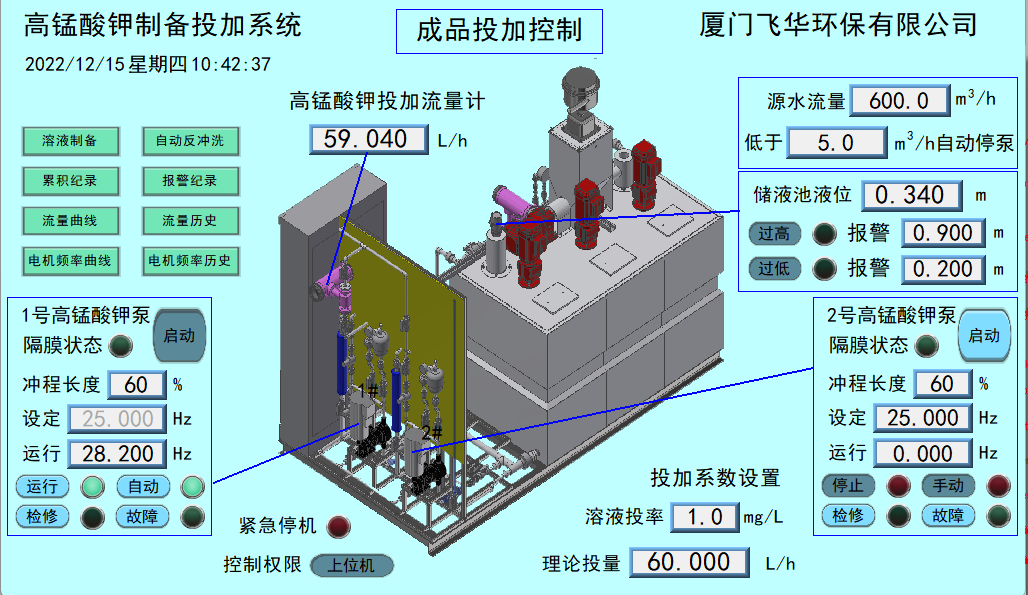
\includegraphics[height=10cm]{g1.PNG}
   \end{figure}
}
\date{}

\maketitle % 封面

\tableofcontents % 目录

\newpage % 换页

%\part{系统组成}
%ctex的\chapter{sdsg}是不能用的
\section{系统组成及功能说明}

   加药装置的主要组成部分,如下图所示:
   \subsection{系统构成图}

      \begin{figure}[h]
         \centering

         \begin{tikzpicture}
            %定义图像
            \node at (0,0) {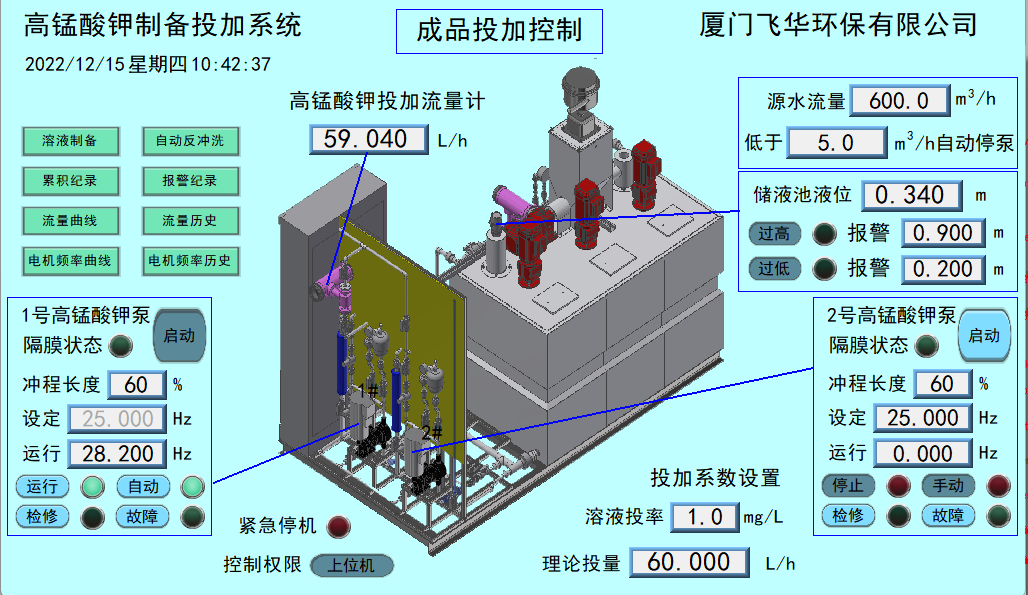
\includegraphics[height=15cm]{g1.PNG}};

            %说明
            \node at (7,1) (1) [text_box] {流量探头};
            \draw [arrow] (1) -- (4.1,-0.2);
            \node at (7,0) (2) [text_box] {计量泵};
            \draw [arrow] (2) -- (5,-1);
            \node at (7,3) (3) [text_box] {阻尼器};
            \draw [arrow] (3) -- (4.3,1.5);
            \node at (4.5,3.5) (4) [text_box] {隔膜压力表};
            \draw [arrow] (4) -- (3.8,1);
            \node at (7,2) (5) [text_box] {可视液位计};
            \draw [arrow] (5) -- (4.6,1);
            \node at (-8,-3) (6) [text_box] {排液阀};
            \draw [arrow] (6) -- (-5.3,-0.8);
            \node at (-8,1) (7) [text_box] {进水阀};
            \draw [arrow] (7) -- (-4.8,0.2);
            \node at (-4,-7) (8) [text_box] {真空上料器风机};
            \draw [arrow] (8) -- (-1,-2.5);
            \node at (-6,-4) (9) [text_box] {Y型过滤器};
            \draw [arrow] (9) -- (-3.8,-0.5);
            \node at (-5,-5) (10) [text_box] {供药阀};
            \draw [arrow] (10) -- (-1.3,-1);
            \node at (7,-5) (11) [text_box] {标定柱};
            \draw [arrow] (11) -- (4.5,-2.5);
            \node at (0,-7) (13) [text_box] {控制电柜};
            \draw [arrow] (13) -- (1,-1);
            \node at (-1,7) (14) [text_box] {搅拌机};
            \draw [arrow] (14) -- (-1,4);
            \node at (5,5) (15) [text_box] {超声波液位计};
            \draw [arrow] (15) -- (0.2,2.3);
            \node at (3,7) (16) [text_box] {搅拌机};
            \draw [arrow] (16) -- (1,3);
            \node at (1,6) (17) [text_box] {螺旋进料器};
            \draw [arrow] (17) -- (-1,2);
            \node at (-8,2) (18) [text_box] {进水流量探头};
            \draw [arrow] (18) -- (-3.8,2);
            \node at (-8,5) (18) [text_box] {进水电动阀};
            \draw [arrow] (18) -- (-3.1,1.8);
            \node at (-8,6) (19) [text_box] {进水压力表};
            \draw [arrow] (19) -- (-2.7,2);
            \node at (-4,7) (20) [text_box] {料斗};
            \draw [arrow] (20) -- (-3,4.5);
            \node at (-6,7) (21) [text_box] {进水压力变送器};
            \draw [arrow] (21) -- (-2.5,2);

			% 辅助线
            \def \xLimit {8};
            \def \yLimit {8};
            
			% 辅助线
            \draw (-\xLimit,-\yLimit) [help lines] grid (\xLimit,\yLimit);
            \foreach \x in {-\xLimit, ...,\xLimit}{
               \node [red] at (\x, \yLimit) {\x};
               \node [red] at (\x, -\yLimit) {\x};
               \node [red] at (\x, 0) {\x};
            }
            \foreach \y in {-\yLimit, ...,\yLimit}
                  \node [red] at (-\xLimit, \y) {\y};
            \foreach \y in {-\yLimit, ...,\yLimit}
                  \node [red] at (\xLimit, \y) {\y};
            \foreach \y in {-\yLimit, ...,\yLimit}
                  \node [red] at (0, \y) {\y};


         \end{tikzpicture}
         \caption{系统组成}
      \end{figure}

\newpage % 换页

      \begin{figure}[h]
         \centering

         \begin{tikzpicture}
         %   \draw (-8,-7) [help lines] grid (8,7);
         %    \draw [red] (-8,0) -- (8,0);
         %    \draw [red] (0,-7) -- (0,7);
            %图片
            \node at (0,0) {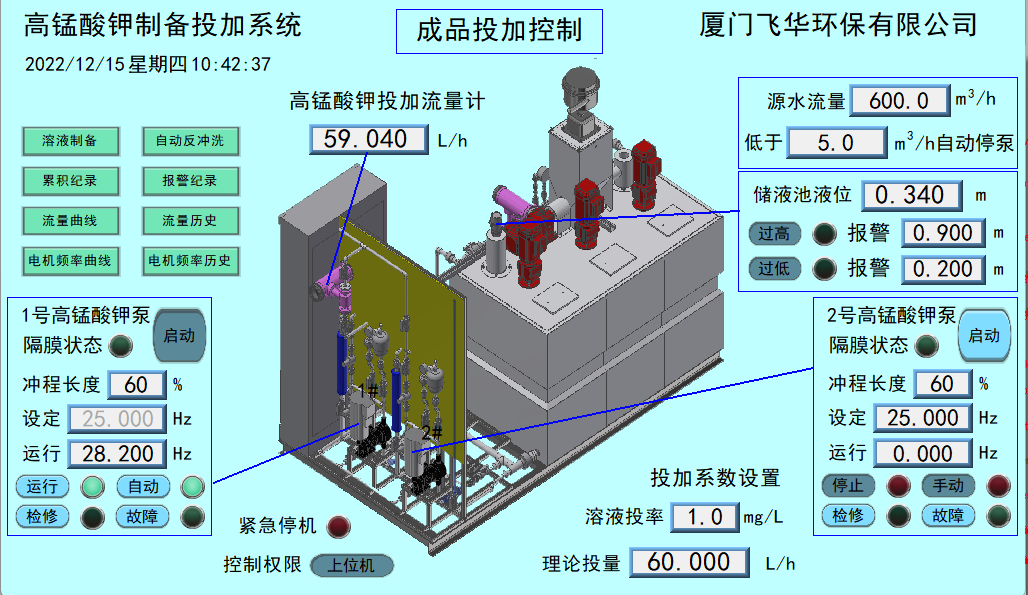
\includegraphics[height=12cm]{g1.PNG}};

            %说明
            \node at (7,5) (1) [text_box] {搅拌机};
            \draw [arrow] (1) -- (4.2,3.5);
            \node at (6,6) (2) [text_box] {料斗};
            \draw [arrow] (2) -- (2.5,3.5);
            \node at (7,-2) (3) [text_box] {搅拌机};
            \draw [arrow] (3) -- (2.5,2.3);
            \node at (6,-3) (4) [text_box] {搅拌机};
            \draw [arrow] (4) -- (1,1.5);
            \node at (1,7) (5) [text_box] {进水电动阀};
            \draw [arrow] (5) -- (1,2.5);
            \node at (-1,6) (6) [text_box] {进水压力表};
            \draw [arrow] (6) -- (0.6,2.8);
            \node at (-3,5) (7) [text_box] {超声波液位计};
            \draw [arrow] (7) -- (0,2);
            \node at (-7,4) (8) [text_box] {电控柜};
            \draw [arrow] (8) -- (-5,2.5);
            \node at (-7,-4) (9) [text_box] {标定柱};
            \draw [arrow] (9) -- (-3.7,-2);
            \node at (-8,1) (9) [text_box] {背压阀};
            \draw [arrow] (9) -- (-3,1);
            \node at (-8,0) (10) [text_box] {安全阀/泄压阀};
            \draw [arrow] (10) -- (-3,-0.3);
            \node at (-6,-5) (11) [text_box] {计量泵};
            \draw [arrow] (11) -- (-2.8,-2);
            \node at (-4,-6) (12) [text_box] {标定柱};
            \draw [arrow] (12) -- (-2.2,-3);
            \node at (0,-6) (13) [text_box] {计量泵};
            \draw [arrow] (13) -- (-1,-2.5);
            \node at (2,-5) (14) [text_box] {流量探头};
            \draw [arrow] (14) -- (-0.5,-1.8);
            \node at (4,-4) (15) [text_box] {阻尼器};
            \draw [arrow] (15) -- (-0.5,-0.3);
         \end{tikzpicture}
         \caption{系统组成}
      \end{figure}

   \subsection{系统功能说明}
      高锰酸钾自动制备投加装置主要分为自动制备系统和自动投加装置2部分组成。
      \par操作人员只需要设定好控制参数,系统将自动运行。
      \subsubsection{自动制备系统功能}
         自动制备系统将高锰酸钾固体粉料制备成溶液。
         \par主要设定参数:
         \begin{itemize}
            \item 溶液制备量。制备系统设计制备能力为1000L/h。
            \item 溶液浓度。常用浓度为1\% -- 2\%。
            \item 溶液密度。以1\%浓度算,溶液密度为1.006g/cm$^{3}$。
            \item 开机液位。储液池液位低于开机液位时,制备系统自动开机。
            \item 停机液位。储液池液位高于停机液位时,制备系统自动停机。
            \item 搅拌机间歇运行参数。搅拌机每运行若干分钟,则停止若干分钟,时长可设置。
            \item 进水低水压。进水压力低于此值制备系统自动停机,出厂设置值为2bar。
         \end{itemize}
         \par制备系统自动运行时,
         控制系统根据进水流量探头反馈,
         通过进水电动阀,
         将进水流量控制在上述设定的溶液制备量上。
         \par同时,控制系统根据上述设定参数,
         按以下公式\ref{powder-in}计算出螺旋进料器进料量(kg/h),
         控制进料器电机变频器,
         使进料量达到设定值。
         \begin{equation}
            \label{powder-in}
            \mbox{进料量}(kg/h) = \mbox{溶液制备量}(L/h) \div \mbox{溶液密度}(g/cm^3) \times \mbox{溶液浓度} (\%)
         \end{equation}
         \par制备系统料斗带有高、低料位报警探头,
         料斗料位过低进会自动停机并发出报警。
         此时应使用真空上料机吸取高锰酸钾原料,
         物料足够时制备系统会恢复自动运行。

      \subsubsection{自动投加系统功能}
         自动投加系统按设定参数向进水总管投加高锰酸钾溶液。
         \par主要设定参数:
         \begin{itemize}
            \item 溶液投率。设计溶液投率为1mg/L,可修改。
            \item 溶液浓度。常用浓度为1\% -- 2\%。
            \item 溶液密度。以1\%浓度算,溶液密度为1.006g/cm$^{3}$。
            \item 源水低水量报警。源水水量低于此设定则自动停泵。
            \item 计量泵轮换设置。计量泵连续运行若干小时,则切换到另1台计量泵运行。
            \item 储液池低液位报警设置。低于此液位高锰酸钾溶液不足,自动停泵。
         \end{itemize}
         \par控制系统按以下公式\ref{chemical-flow}计算的流量,
         控制计量泵变频器,
         向进水总管投加制备好的高锰酸钾溶液。
         \begin{equation}
            \label{chemical-flow}
            \mbox{投加流量}(L/h) = \mbox{溶液投率}(mg/L) \times 
            \mbox{源水水量}(m^3/h) \div 
            \mbox{溶液密度}(g/cm^3) \div 
            \mbox{溶液浓度}(\%)
         \end{equation}


\newpage % 换页

\section{设备启动前准备}\label{sec:sg1}
   \subsection{紧固件检查}
      系统启动前,要先对所有的紧固件进行检查。
      紧固件包括底座固定螺栓、泵固定螺栓、马达连接螺栓以及所有的法兰连接螺栓等。
      如有松动情况,请将其上紧,如有脱落等情况,请按相应的规格补充相关的螺栓。

   \subsection{管道连接检查}
      检查管道中所有活接接头连接,如有松脱情况需要重新上紧。

   \subsection{检查系统中各阀门状态}
      \subsubsection{各检修阀门应处于关闭状态}\label{sec:sg3}
         检修阀门包括检修排液阀、检修旁通阀等,
         正常运行时均应处于关闭状态。
      \begin{figure}[h]
         \centering
         \begin{tikzpicture}
            % \draw (-7,-6) [help lines] grid (7,6);
            % \draw [red] (-7,0) -- (7,0);
            % \draw [red] (0,-6) -- (0,6);
            %图片
            \node at (0,0) {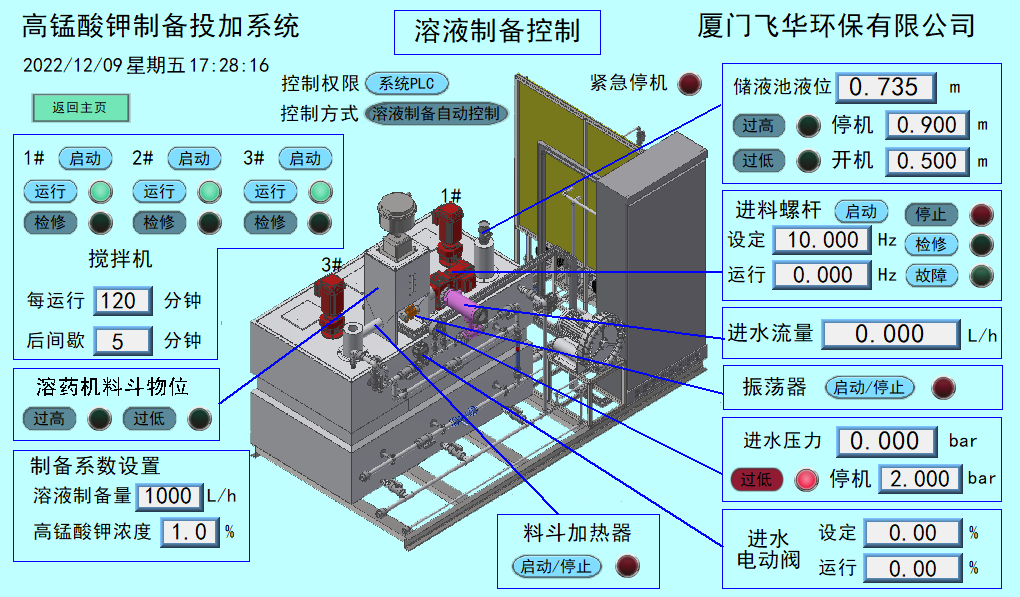
\includegraphics[height=12cm]{g2.PNG}};

            %说明
            \node at (-6,-4) (1) [text_box] {检修排液阀};
            \draw [arrow] (1) -- (-1,-2.1);
            \draw (-1,-2.1) circle (0.5)[red];
            \node at (6,-4) (2) [text_box] {检修排液阀};
            \draw [arrow] (2) -- (2,-2.1);
            \draw (2,-2.1) circle (0.5)[red];
         \end{tikzpicture}
         \caption{检修排液阀位置}\label{fig:g3}
      \end{figure}

\newpage

      \begin{figure}[h]
         \centering
         \begin{tikzpicture}
            % \draw (-7,-6) [help lines] grid (7,6);
            % \draw [red] (-7,0) -- (7,0);
            % \draw [red] (0,-6) -- (0,6);
            %图片
            \node at (0,0) {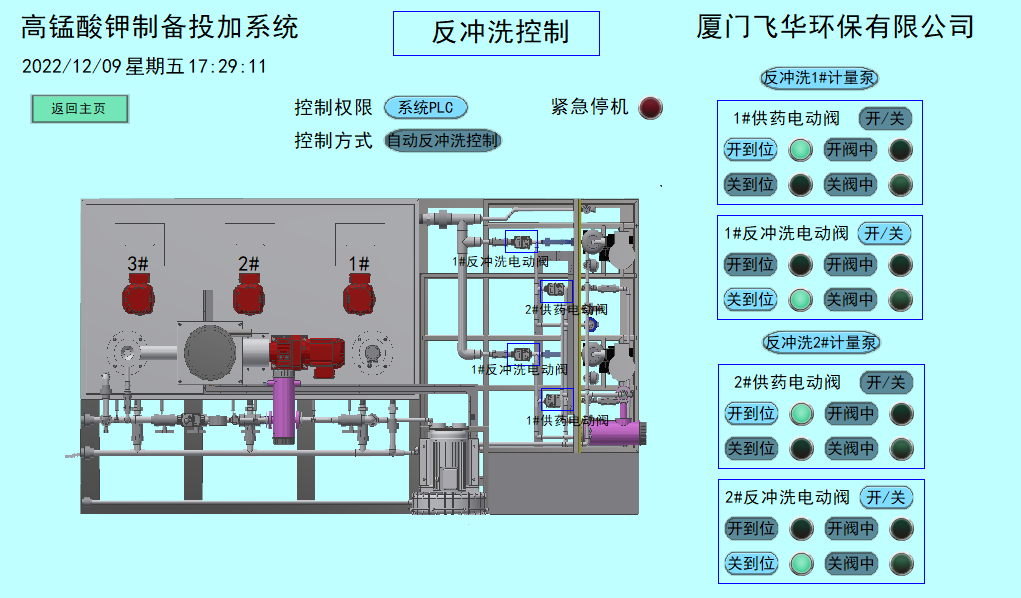
\includegraphics[height=12cm]{g3.PNG}};

            %说明
            \node at (5,-5) (1) [text_box] {检修排液阀};
            \draw [arrow] (1) -- (-0.2,-3.3);
            \draw (-0.2,-3.3) circle (0.5)[red];
            \node at (6,-4) (2) [text_box] {检修排液阀};
            \draw [arrow] (2) -- (1.3,-2.3);
            \draw (1.3,-2.3) circle (0.5)[red];
            \node at (4,-6) (3) [text_box] {检修排液阀};
            \draw [arrow] (3) -- (-1.9,-4.2);
            \draw (-1.9,-4.2) circle (0.5)[red];
            \node at (-5,-6) (4) [text_box] {检修旁通阀};
            \draw [arrow] (4) -- (-0.6,-1.6);
            \draw (-0.6,-1.6) circle (0.5)[red];
         \end{tikzpicture}
         \caption{检修排液阀、旁通阀位置}\label{fig:g4}
      \end{figure}
      \par上图\ref{fig:g3}和图\ref{fig:g4}所示为检修排液阀、检修旁通阀所在位置。
      % \par表示这是一段,新开一段才会自动退2个空格
      \par检修排液阀的作用,
      用于在检修时释放系统压力,
      避免管道内化学品喷射出来。
      \par检修旁通阀的作用,
      是流量探头、电动阀、压力变送器、压力表等需要检修时,
      关闭其上下游阀门,
      打开检修旁通阀,
      可在手动状态维持系统运行。
      \par正常工作时应将检修排液阀、检修旁通阀关闭。

\newpage % 换页

      \subsubsection{标定柱控制阀应处于关闭状态}
      \begin{figure}[h]
         \centering
         \begin{tikzpicture}
            % \draw (-7,-6) [help lines] grid (7,6);
            % \draw [red] (-7,0) -- (7,0);
            % \draw [red] (0,-6) -- (0,6);
            %图片
            \node at (0,0) {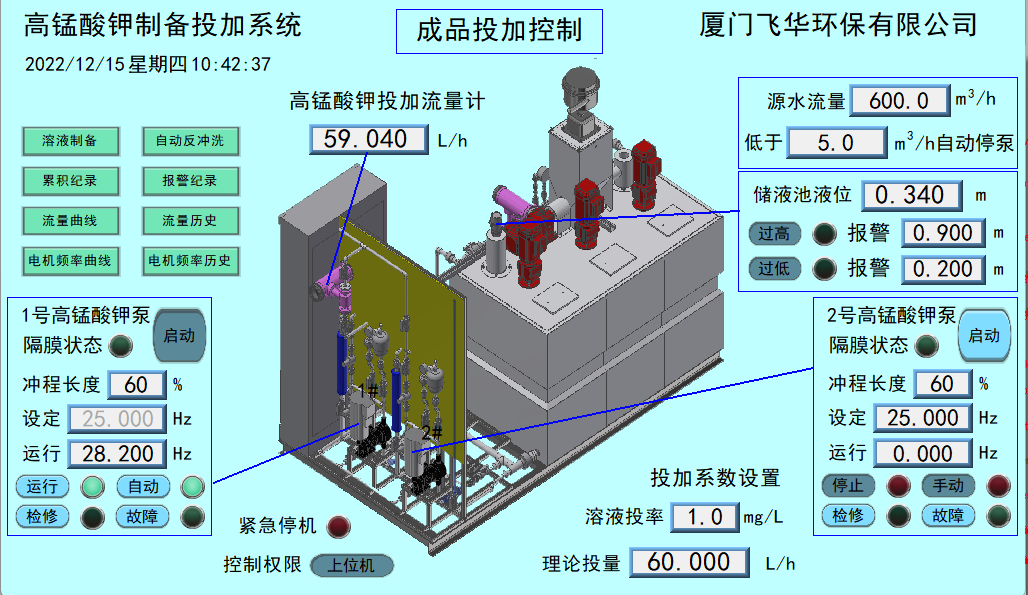
\includegraphics[height=12cm]{g1.PNG}};

            %说明
            \node at (3,-5) (1) [text_box] {标定柱控制阀};
            \draw [arrow] (1) -- (-1.8,-3.7);
            \draw (-1.8,-3.7) circle (0.5)[red];
            \node at (-6,-5) (2) [text_box] {标定柱控制阀};
            \draw [arrow] (2) -- (-3.3,-2.8);
            \draw (-3.3,-2.8) circle (0.5)[red];
         \end{tikzpicture}
         \caption{标定柱控制阀位置}\label{fig:g5}
      \end{figure}

      上图\ref{fig:g5}所示为标定柱控制阀所在位置。
      图中标定柱控制阀为打开状态,系统启动前应将其关闭。
      \par标定柱的作用是校正流量监控仪表以及确定计量泵真实流量,
      进行流量标定时应将标定柱控制阀,正常工作时应将其关闭。\\
\subsubsection{其余阀门均处于开启状态}
      除上述特别说明之外的所有阀门,在正常工作状态下,都应处于开启状态。

\newpage % 换页

\section{日常操作}
   \subsection{制备投加系统上电}
      \subsubsection{电柜操作面板布局}
         电柜操作面板布局如下图\ref{fig:g7}:
         \begin{figure}[h]
            \centering
            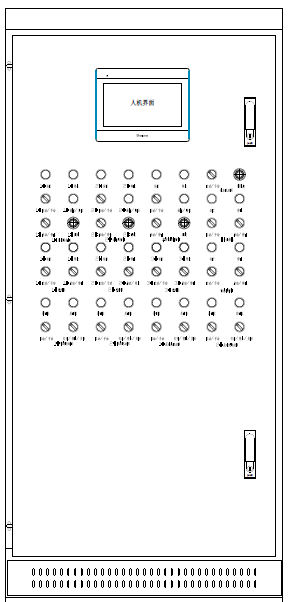
\includegraphics[height=12cm]{g5.png}
            \caption{电柜操作面板布局图}\label{fig:g7}
         \end{figure}
         \newline
         \par电柜操作面板包括人机界面、控制开关、控制旋扭及指示灯,
         用于展示加药装置运行状态和设备控制。
         \par一般日常操作,
         在人机界面设定相应的运行参数,
         制备投加系统则会自动运行。
         \par因此,除检修和维护设备的情况外,
         建议将计量泵、搅拌机、阀门的手动/自动切换开关都调到”自动“状态,
         由控制系统自动控制。
         \par振荡器和加热器,
         是在螺旋进料器运行不顺畅时使用,
         建议手动启停。

         \newpage

      \subsubsection{电柜布局}
         电柜布局如下图\ref{fig:g6},开关区域位置电柜内左上角。
         \begin{figure}[h]
            \centering
               \begin{tikzpicture}
                  % \draw (-7,-8) [help lines] grid (7,8);
                  % \draw [red] (-7,0) -- (7,0);
                  % \draw [red] (0,-8) -- (0,8);
                  %图片
                  \node at (0,0) {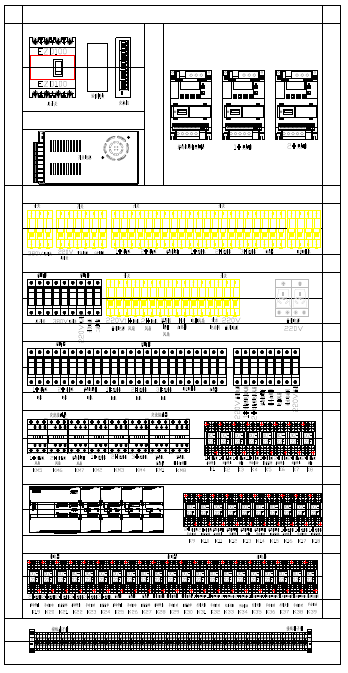
\includegraphics[height=16cm]{g4.PNG}};

                  %说明
                  \node at (-6,4) (1) [text_box] {电柜总开关};
                  \draw [arrow] (1) -- (-3,6);
                  \draw (-3.5,5.5) rectangle +(1.3,1.8)[red];
                  \node at (-6,2) (2) [text_box] {开关区域};
                  \draw [arrow] (2) -- (0,2.5);
                  \draw [arrow] (2) -- (0,1);
                  \draw (-3.5,1.8) rectangle +(7,1.5)[red];
                  \draw (-1.8,0.2) rectangle +(3.5,1.3)[red];
               \end{tikzpicture}
            \caption{电柜布局图}\label{fig:g6}
         \end{figure}

      \subsubsection{依次打各开关}
      打开总电源开关。
      \par依次打开380V总开关、风扇、开关电源、二次回路等总开关。
      \par依次打开计量泵、溶药机螺杆、搅拌机、真空吸料机、电机风扇、电柜风扇、进水电动阀等开关。
      \par振荡器、料斗加热器开关可在需要使用时打开。

      \subsubsection{观察加药装置各系统状态}
      观察人机界面、变频器、PLC及流量仪表工作状态是否正常。
      在正常情况下,人机界面、变频器及流量仪表显示器均应该点亮,PLC上应无红灯闪烁。

      \subsubsection{异常情况处理}
      加药系统上电如发现异常情况,请与加药系统售后服务人员联系。
      如需自行处理,请先详细查阅附件技术资料,自行处理若操作不当,有可能导致加药系统损坏。

   \subsection{主控制界面}\label{sec:s1}
      自动制备投加系统主要通过人机界面设定系统运行参数。
      \par人机界面的主控制界面如下图\ref{fig:g7}所示。
      \par主控制界面可以切换到其他控制界面,
      下图\ref{fig:g7}红圈内为切换到其他控制界面的区域。
      \par同时,主控制界面设置高锰酸钾投加系统的运行参数。

      \begin{figure}[h]
         \centering
            \begin{tikzpicture}
               % \draw (-8,-4) [help lines] grid (8,4);
               % \draw [red] (-8,0) -- (8,0);
               % \draw [red] (0,-4) -- (0,4);
               %图片
               \node at (0,0) {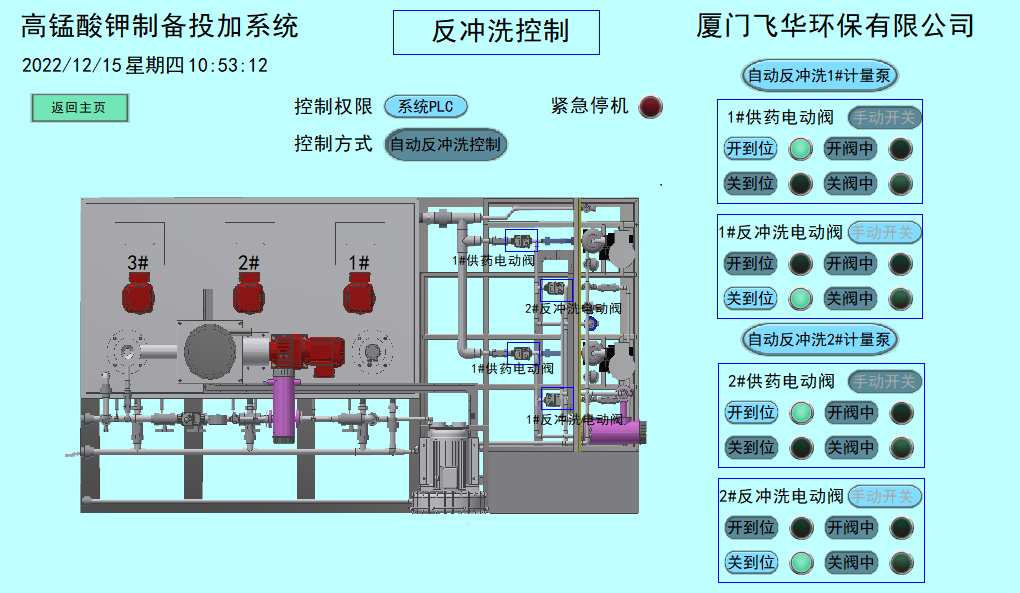
\includegraphics[height=8cm]{g6.PNG}};

               %说明
               \node at (-2,3) (1) [text_box, color=red] {界面切换区域};
               % \draw [arrow] (1) -- (-3,6);
               \draw (-6.8,0.5) rectangle +(5,2.2)[red];
            \end{tikzpicture}
         \caption{主控制界面}\label{fig:g7}
      \end{figure}

   \subsection{设置制备系统参数}\label{sec:sg5}
      制备系统开始运行前,
      要先设置好制备系统运行参数。
      \par在上图\ref{fig:g7}主控制界面上,
      按”溶液制备“按钮,
      切换到溶液制备控制界面。
      \par或者按”搅拌机控制“按钮,
      切换到搅拌机控制界面。
      \par制备系统运行参数设置好之后,
      将会自动运行,
      无须人工参与。
      出现供水水压过低,
      或料斗料位过低,
      制备系统将自动停机。

      \newpage

      \begin{figure}[h]
         \centering
            \begin{tikzpicture}
               % \draw (-8,-4) [help lines] grid (8,4);
               % \draw [red] (-8,0) -- (8,0);
               % \draw [red] (0,-4) -- (0,4);
               %图片
               \node at (0,0) {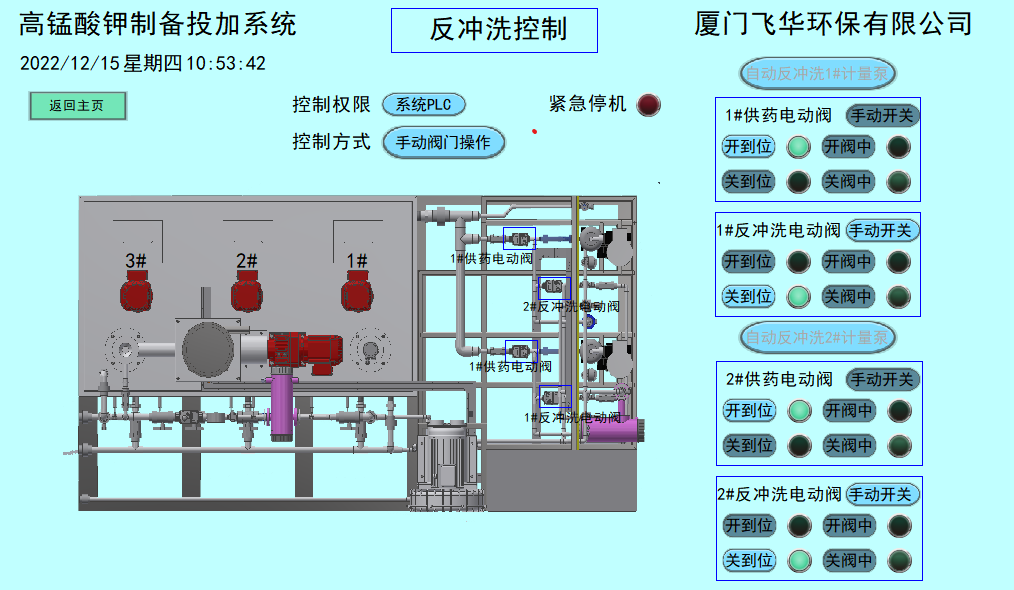
\includegraphics[height=8cm]{g7.PNG}};

               %说明
               \node at (-1,3) (1) [text_box, color=red] {切换到搅拌机控制};
               \draw [arrow, color=red] (1) -- (-4,2.5);
               \node at (-4,2) (1) [text_box, color=red] {参数1};
               \node at (5.9,2.6) (1) [text_box, color=red] {参数2};
               \node at (5.9,-0.9) (1) [text_box, color=red] {参数3};
            \end{tikzpicture}
         \caption{溶液制备控制界面}\label{fig:g8}
            \begin{tikzpicture}
               % \draw (-8,-4) [help lines] grid (8,4);
               % \draw [red] (-8,0) -- (8,0);
               % \draw [red] (0,-4) -- (0,4);
               %图片
               \node at (0,0) {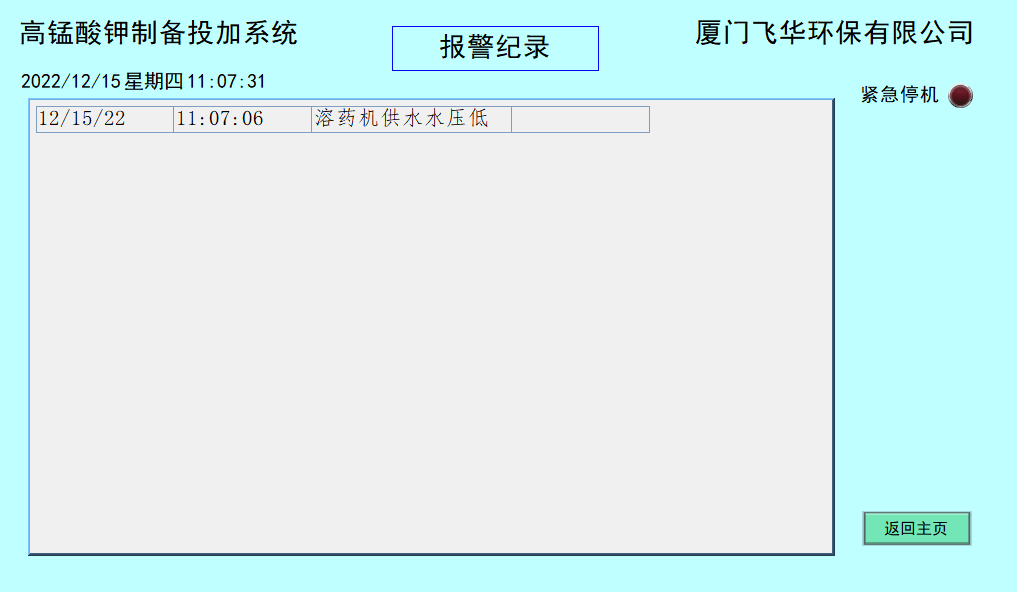
\includegraphics[height=8cm]{g8.PNG}};

               %说明
               \node at (-2,3) (1) [text_box, color=red] {切换到溶液制备};
               \draw [arrow, color=red] (1) -- (-4,2.5);
               \node at (-4.5,-0.5) (1) [text_box, color=red] {参数4};
            \end{tikzpicture}
         \caption{搅拌机控制界面}\label{fig:g9}
      \end{figure}

      \par在上图\ref{fig:g8}以及图\ref{fig:g9}界面设置好以下参数:
      \begin{enumerate}
         \item 制备系数。
            \begin{itemize}
               \item 溶液制备量。制备系统设计制备能力为1000L/h。
               \item 高锰酸钾浓度。常用浓度为1\% -- 2\%,默认设置为1\%。
               \item 溶液密度。以1\%浓度算,溶液密度为1.006g/cm$^{3}$。
            \end{itemize}
         \item 开机、停机液位。
            \begin{itemize}
               \item 开机液位。储液池液位低于开机液位时,制备系统自动开机,默认0.5m。
               \item 停机液位。储液池液位高于停机液位时,制备系统自动停机,默认0.9m。
            \end{itemize}
         \item 低水压停机值。进水压力低于此值制备系统自动停机,出厂设置值为2bar。
         \item 搅拌机间歇运行参数。搅拌机每运行若干分钟,则停止若干分钟。
            \begin{itemize}
               \item 运行时长。默认30min。
               \item 间歇时长。默认5min。
            \end{itemize}
      \end{enumerate}
      

   \subsection{制备系统供水、上料}
      \subsubsection{制备系统供水}\label{sec:sg2}
         连接制备系统供水管道,
         确认供水压力高于低水压停机值(出厂设定为2bar)。
         如果供水压力低于低水压停机值,
         制备系统会自动停机。
      \begin{figure}[h]
         \centering
            \begin{tikzpicture}
               % \draw (-8,-4) [help lines] grid (8,4);
               % \draw [red] (-8,0) -- (8,0);
               % \draw [red] (0,-4) -- (0,4);
               %图片
               \node at (0,0) {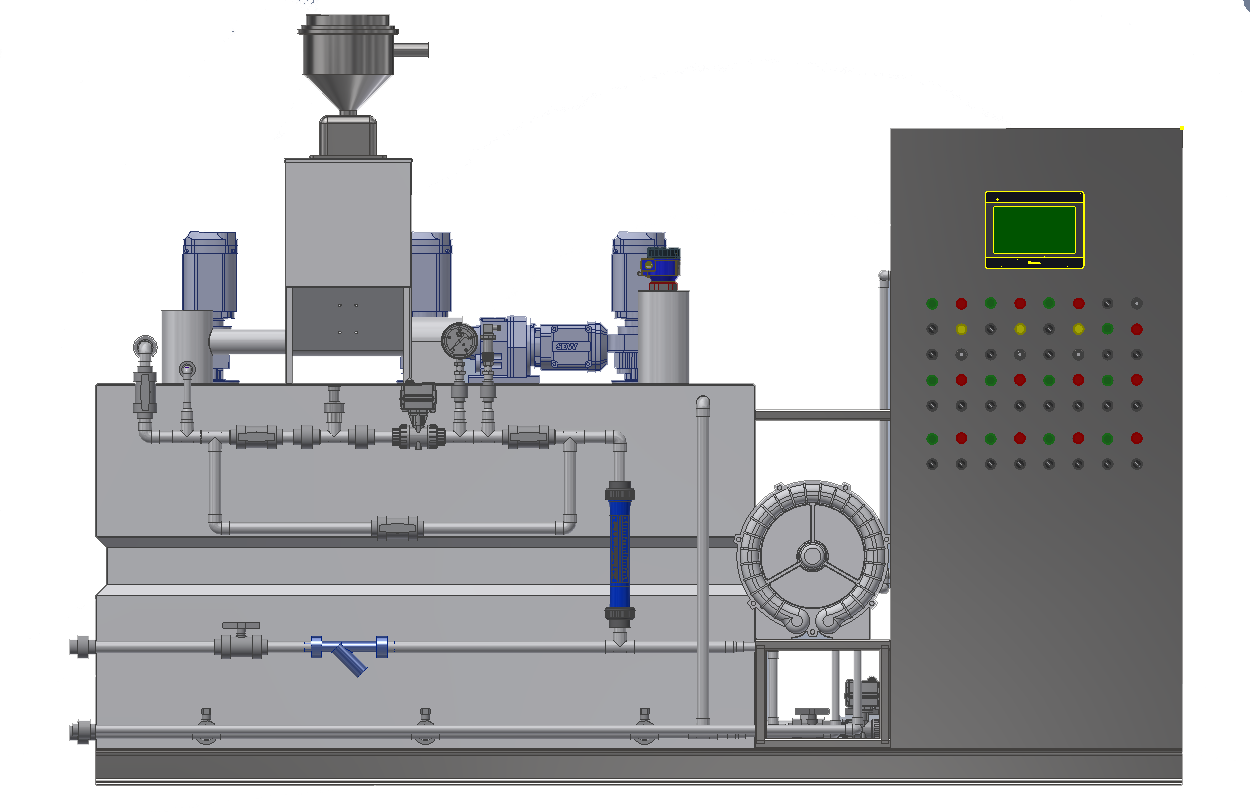
\includegraphics[height=8cm]{g9.PNG}};

               %说明
               \node at (-8,-3) (1) [text_box] {进水管};
               \draw [arrow] (1) -- (-5.2,-2.3);
               \draw (-5.2,-2.3) circle (0.5)[red];
               \node at (4,4) (2) [text_box] {进水压力表及压力变送器};
               \draw [arrow] (2) -- (-1.5,0.5);
               \draw (-1.5,0.5) circle (0.5)[red];
               \node at (-6,3) (3) [text_box] {进水流量探头};
               \draw [arrow] (3) -- (-2.8,0);
               \draw (-2.8,0) circle (0.5)[red];
               \node at (7,-3) (4) [text_box] {转子流量计};
               \draw [arrow] (4) -- (0,-1.5);
               \draw (0,-1.5) circle (0.5)[red];
               \node at (7,2) (5) [text_box] {真空上料机};
               \draw [arrow] (5) -- (2,-1.5);
               % \draw (2,-1.5) circle (0.5)[red];
            \end{tikzpicture}
         \caption{制备系统供水说明}\label{fig:g10}
      \end{figure}

      \subsubsection{制备系统上料}
         制备系统正常运行,
         需要保证料斗内有足够高锰酸钾粉料,
         料斗内有物位探头,
         料位过低,
         制备系统则自动停机。
         \par料斗内原料不足时,
         应使用真空上料机(参考\ref{sec:sg2}的图\ref{fig:g10}),
         向料斗内补充原料。

         \par启动真空上料机操作流程如下:
         \begin{enumerate}
            \item 打开真空上料机电源开关。见下图\ref{fig:g11}。
            \item 将吸料嘴伸入高锰酸钾粉料包装内。见下图\ref{fig:g11}。
            \item 按run/stop按钮启动真空上料机。
            启动真空上料机之后,
            上料机会自动运行/停止/运行间歇运行,
            方便已经吸上的粉料落入料斗内,
            过程中无须人工干预。见下图\ref{fig:g11}。
            \item 上料过程中应通过人机界面观察料斗内料位状态。见下图\ref{fig:g12}。
         \end{enumerate}

         \begin{figure}[h]
            \centering
               \begin{tikzpicture}
                  % \draw (-8,-4) [help lines] grid (8,4);
                  % \draw [red] (-8,0) -- (8,0);
                  % \draw [red] (0,-4) -- (0,4);
                  %图片
                  \node [rotate=-90] at (0,0) {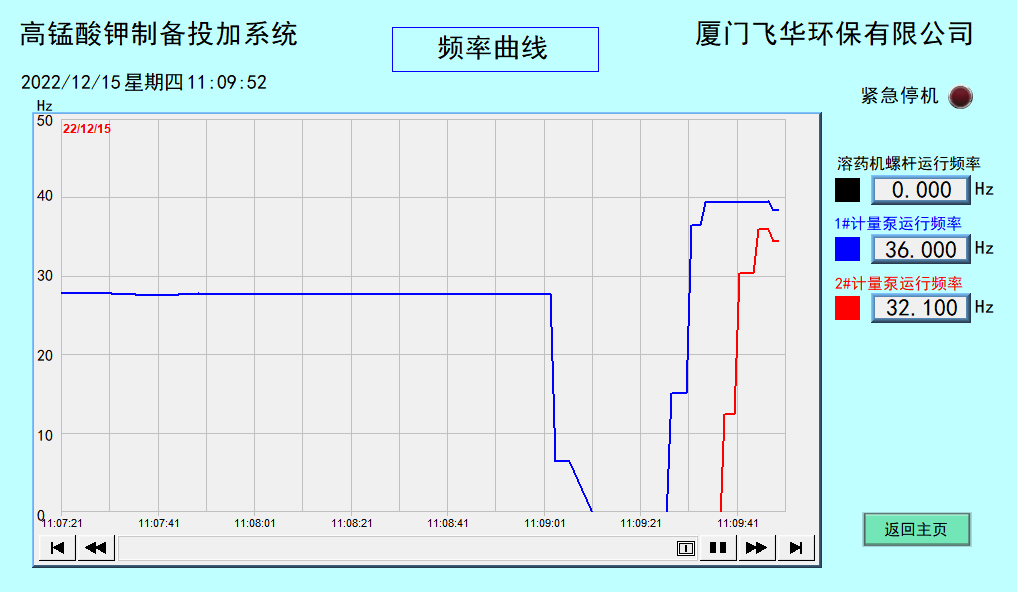
\includegraphics[height=6.6cm]{g10.PNG}};

                  %说明
                  \node at (-6,-2) (1) [text_box] {吸料嘴};
                  \draw [arrow] (1) -- (-2,0.7);
                  \draw (-2,0.7) circle (0.5)[red];
                  \node at (6,-2) (4) [text_box] {run/stop按钮};
                  \draw [arrow] (4) -- (-0.4,0.4);
                  \draw (-0.4,0.4) circle (0.3)[red];
                  \node at (6,3) (5) [text_box] {电源开关};
                  \draw [arrow] (5) -- (1.5,1);
                  \draw (1.5,1) circle (0.8)[red];
               \end{tikzpicture}
            \caption{真空上料机结构说明}\label{fig:g11}
         % \end{figure}

         % \begin{figure}[h]
         %    \centering
               \begin{tikzpicture}
                  % \draw (-8,-4) [help lines] grid (8,5);
                  % \draw [red] (-8,0) -- (8,0);
                  % \draw [red] (0,-4) -- (0,4);
                  %图片
                  \node at (0,0) {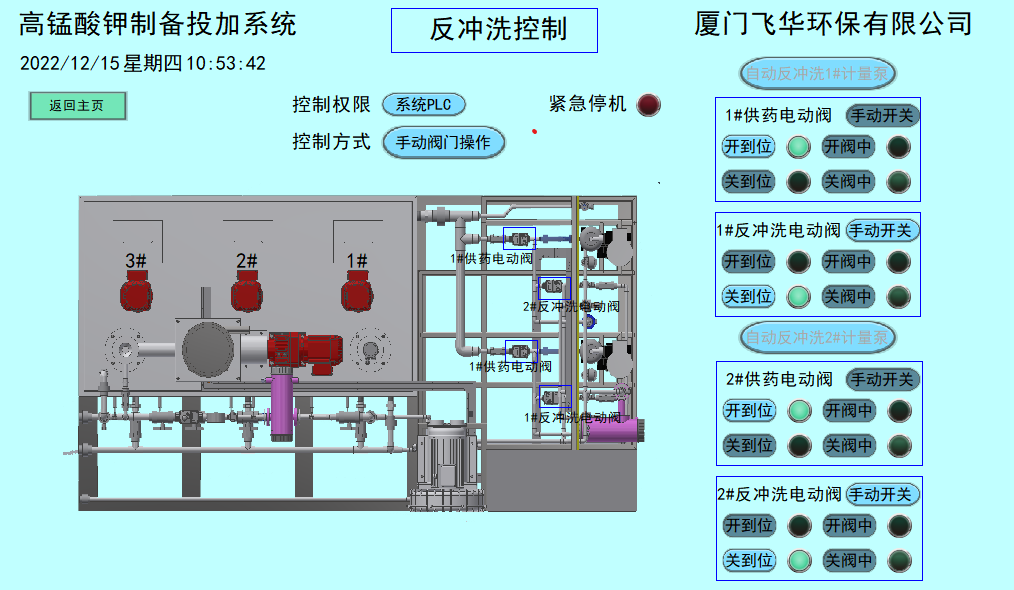
\includegraphics[height=8cm]{g7.PNG}};

                  %说明
                  \node at (-2.5,2) (1) [text_box, color=red] {料斗料位};
                  \draw [arrow, color=red] (1) -- (-5,-0.2);
                  \draw (-6.8,-0.9) rectangle +(3.3,1.2)[red];
               \end{tikzpicture}
            \caption{溶液制备控制界面}\label{fig:g12}
         \end{figure}

         \newpage

            已经吸入足够粉料,或料斗料位探头高报警,则应停止真空上料机。见上图\ref{fig:g12}。
         \par停止真空上料机操作流程如下:
         \begin{enumerate}
            \item 按run/stop按钮启动真空上料机。见上图\ref{fig:g11}。
            \item 将吸料嘴伸入高锰酸钾粉料包装内。见上图\ref{fig:g11}。
            \item 打开真空上料机电源开关。见上图\ref{fig:g11}。
         \end{enumerate}

   \subsection{设置投加系统参数}
        投加系统运行参数设置好之后,
        系统将会自动按相应参数向进水总管投加高锰酸钾,
        无须人工参与。
        \par源水流量过低,
        或储液池液位过低,
        制备系统将自动停机。

        \begin{figure}[h]
            \centering
                \begin{tikzpicture}
                %图片
                \node at (0,0) {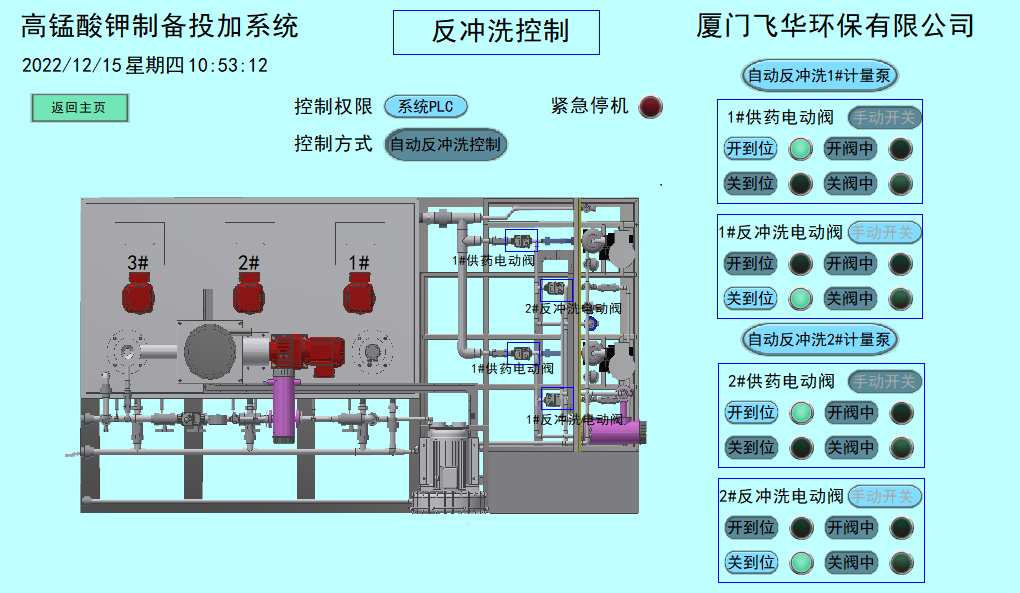
\includegraphics[height=8cm]{g6.PNG}};

                %说明
                \node at (-4.2,0.2) (1) [text_box, color=red] {参数1};
                \node at (4.3,2.3) (2) [text_box, color=red] {参数2};
                \node at (5.5,0.6) (3) [text_box, color=red] {参数2};
                \node at (-2.2,-3.6) (4) [text_box, color=red] {参数3};
                \node at (5.4,-1.8) (5) [text_box, color=red] {参数4};
                \node at (-5.2,-1.8) (6) [text_box, color=red] {参数4};

                %坐标辅助线
                % \draw (-8,-4) [help lines] grid (8,4);
                % \draw [red] (-8,0) -- (8,0);
                % \draw [red] (0,-4) -- (0,4);
                \end{tikzpicture}
            \caption{成品投加控制界面}\label{fig:g13}
        \end{figure}

      \par在上图\ref{fig:g13}界面设置以下参数:
      \begin{enumerate}
         \item 投加系数。
            \begin{itemize}
                \item 溶液投率。设计溶液投率为1mg/L即每L源水投加1mg高锰酸钾固体。
                \item 溶液密度。以1\%浓度算,溶液密度为1.006g/cm$^{3}$。
                \item 高锰酸钾浓度。在溶液制备参数中已设置(见\ref{sec:sg5}第\pageref{sec:sg5}页),此处无须再设置。
            \end{itemize}
         \item 停泵条件。
            \begin{itemize}
               \item 源水低流量。源水流量过低,投加系统自动停泵,默认5m$^{3}$/h。
               \item 储液池低液位。储液池液位过低时,投加系统自动停泵,默认0.2m。
            \end{itemize}
        \item 计量泵轮换设置。计量泵连续运行若干小时,则切换到另1台计量泵运行,默认8小时。
        \item 计量泵冲程长度。计量泵当前冲程长度,默认是60\%,如要修改请参考计量泵操作说明。
      \end{enumerate}

    \subsection{累积记录、报警记录、运行曲线、历史数据}
        高锰酸钾自动制备投加系统运行状态监控界面有累积记录、报警记录、运行曲线等、历史数据。
        \par上述几个界面,
        均可从主控制界面进入,
        参考\ref{sec:sg1}第\pageref{sec:sg1}页图\ref{fig:g7}。

        \subsubsection{累积记录}
            \begin{figure}[h]
                \centering
                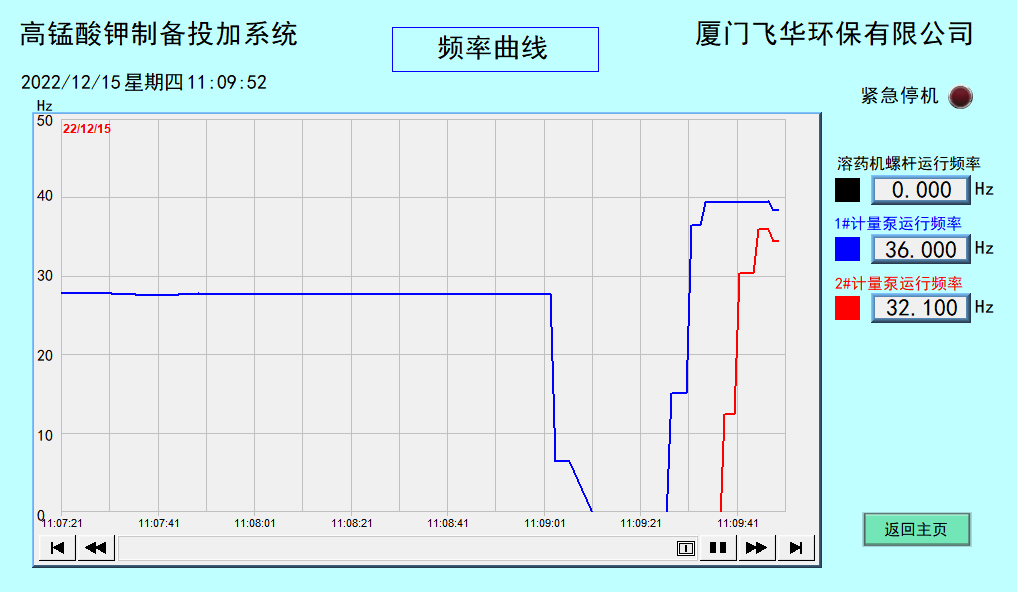
\includegraphics[height=6cm]{g10.PNG}
                \caption{累积纪录}\label{fig:g14}
            \end{figure}
            
        \subsubsection{报警记录}
            \begin{figure}[h]
                \centering
                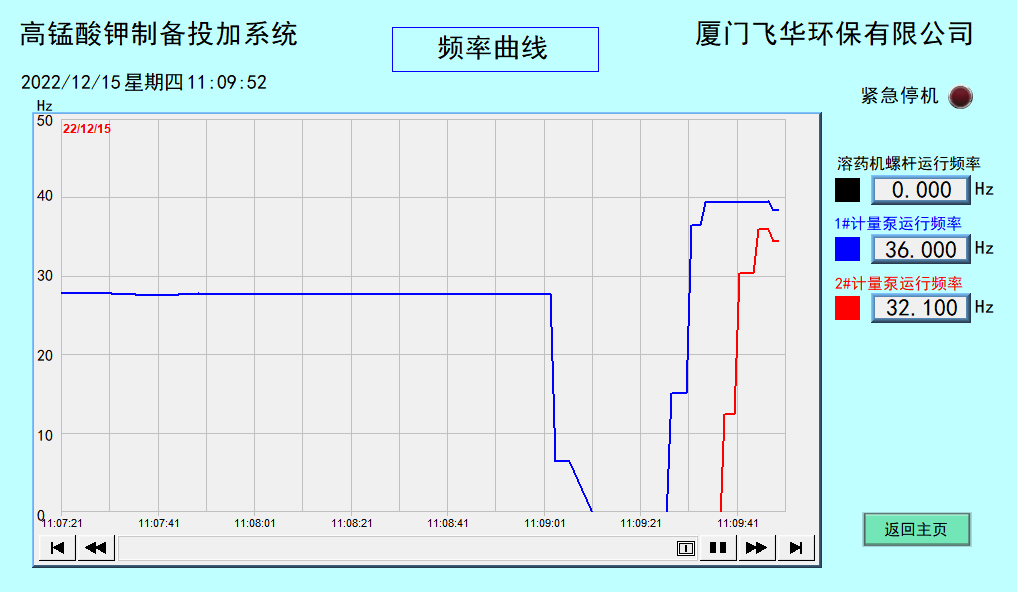
\includegraphics[height=6cm]{g10.PNG}
                \caption{报警记录}\label{fig:g15}
            \end{figure}

        \newpage

        \subsubsection{运行曲线}
            \begin{figure}[h]
                \centering
                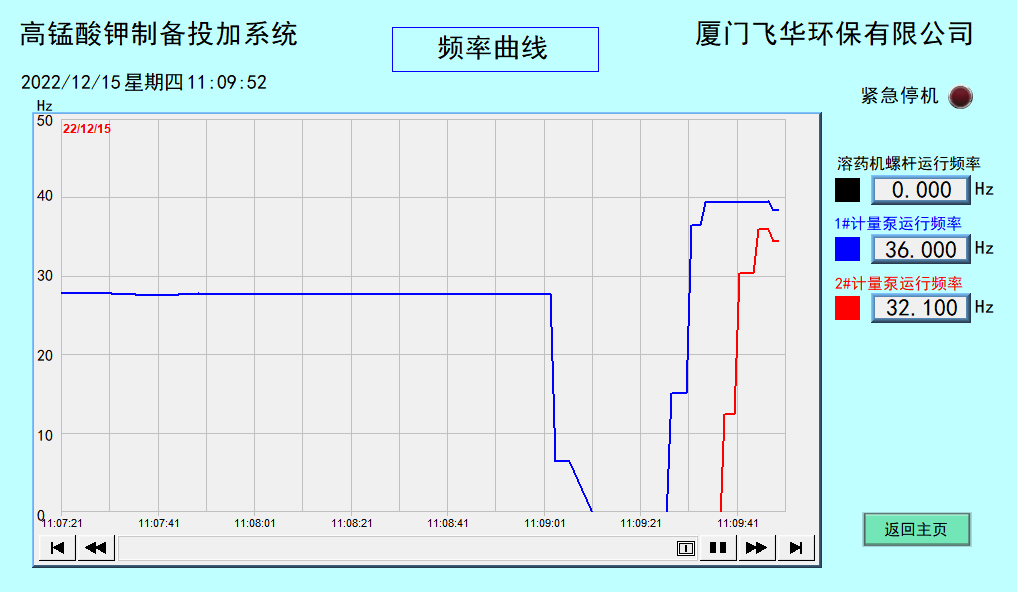
\includegraphics[height=6cm]{g10.PNG}
                \caption{加药流量曲线}\label{fig:g16}
               \quad\\ 
                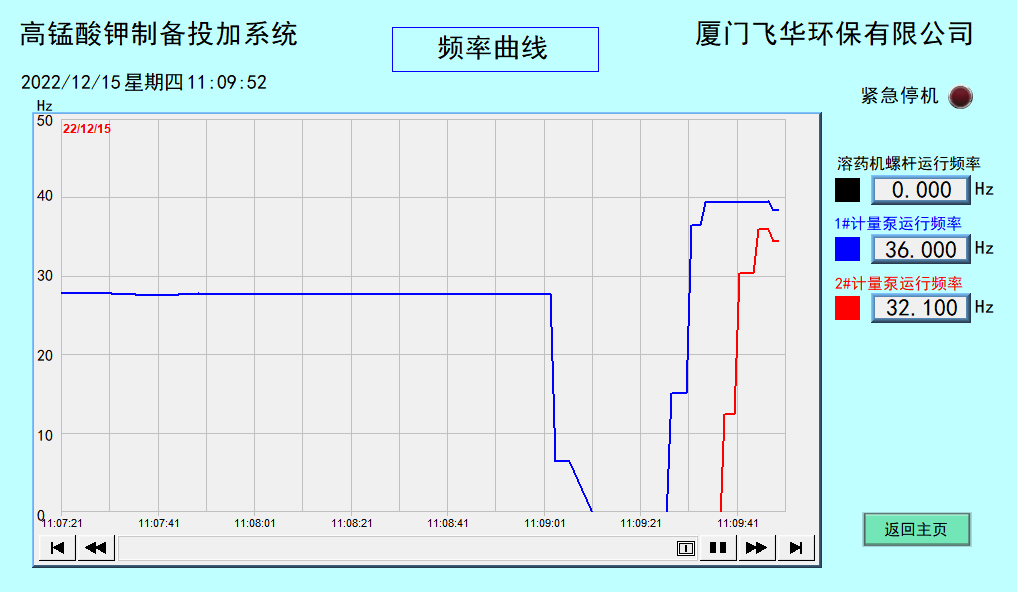
\includegraphics[height=6cm]{g10.PNG}
                \caption{电机频率曲线}\label{fig:g17}
            \end{figure}

\section{维护及检修}
   建议联系加药系统经销商及售后服务人员,
   由专业人士进行维护及检修,
   如自行进行维护及检修,
   有可能导致制备投加装置损坏。
   \par维护及检修之前,
   请先阅读下文,
   以及计量泵的操作说明书。
   下文内容为加药装置维护及检修操作方法。

   \subsection{制备系统的检修维护}
        \subsubsection{传感器及电动阀的检修维护} 
            制备系统的传感器有进水压力变送器、
            进水压力表、进水电动阀、
            进水流量探头、储液槽超声波液位计、
            料斗高低料位探头等。

            \newpage

            \begin{figure}[h]
                \centering
                \begin{tikzpicture}
                    %图片
                    \node at (0,0) {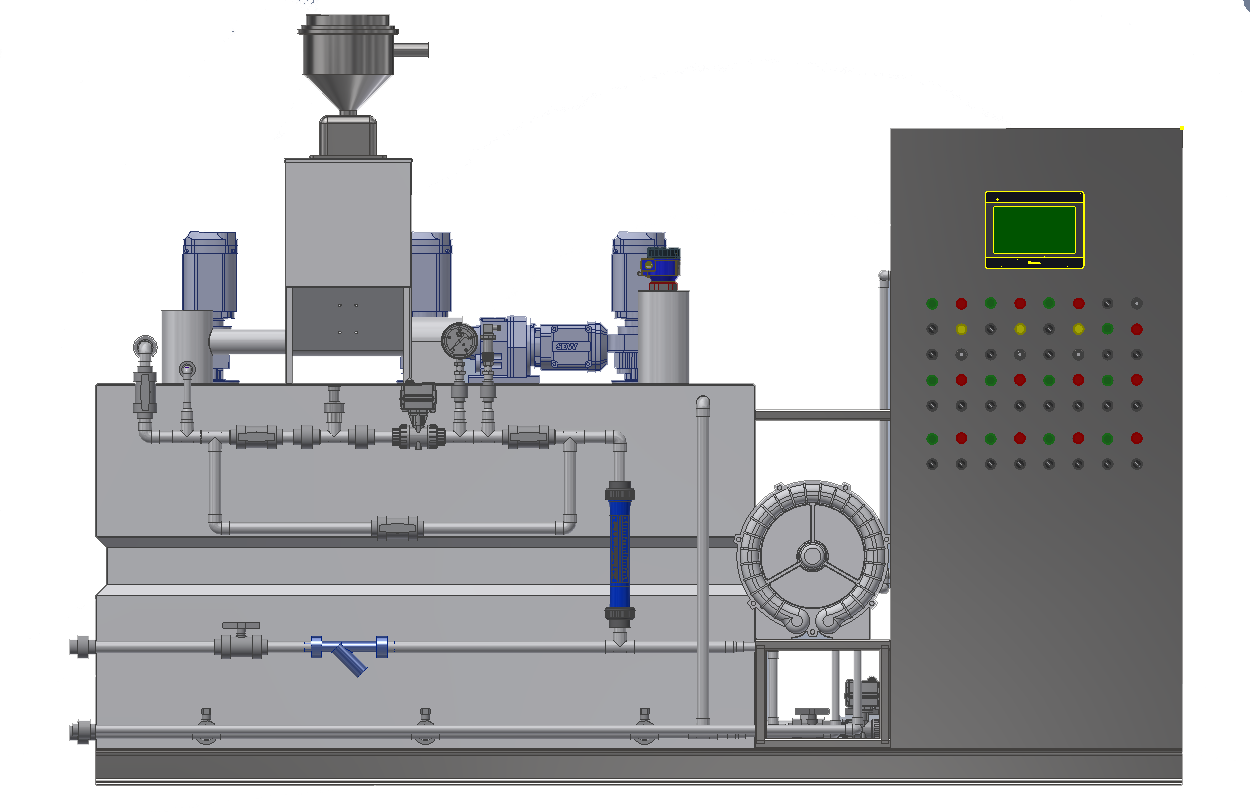
\includegraphics[height=10cm]{g9.PNG}};

                    %说明
                    \node at (-7,2) (2) [text_box] {进水流量探头};
                    \draw [arrow] (2) -- (-3.5,0);
                    \draw (-3.5,0) circle (0.5)[red];
                    \node at (0,3) (1) [text_box] {检修截止阀};
                    \draw [arrow] (1) -- (-1.2,-0.4);
                    \draw (-1.2,-0.4) circle (0.5)[red];
                    \node at (-8,-3) (3) [text_box] {检修旁通阀};
                    \draw [arrow] (3) -- (-2.7,-1.5);
                    \draw (-2.7,-1.5) circle (0.5)[red];
                    \node at (-8,1) (4) [text_box] {检修截止阀};
                    \draw [arrow] (4) -- (-4.5,-0.4);
                    \draw (-4.5,-0.4) circle (0.5)[red];
                    \node at (-6,3) (5) [text_box] {进水电动阀};
                    \draw [arrow] (5) -- (-2.5,0);
                    \draw (-2.5,0) circle (0.5)[red];
                    \node at (-1,4) (6) [text_box] {进水压力表及变送器};
                    \draw [arrow] (6) -- (-1.8,0.8);
                    \draw (-1.8,0.8) circle (0.5)[red];
                    \node at (3,5) (7) [text_box] {超声波液位计};
                    \draw [arrow] (7) -- (0.5,1.5);
                    \draw (0.5,1.5) circle (0.5)[red];
                    \node at (5,4) (8) [text_box] {超声波液位计安装座};
                    \draw [arrow] (8) -- (0.5,0.5);
                    \draw (0.5,0.5) circle (0.5)[red];

                    %辅助线
                    % \draw (-8,-5) [help lines] grid (8,5);
                    % \draw [red] (-8,0) -- (8,0);
                    % \draw [red] (0,-5) -- (0,5);
                \end{tikzpicture}
                \caption{主要传感器及电动阀位置}
            \end{figure}

            \par 检修进水流量探头、
            进水电动阀、
            进水压力表、
            进水压力变送器之前,
            应先关闭上下游检修截止阀,
            并打开检修旁通阀。
            \par 拆下
            超声波液位计安装座, 
            即可检修
            超声波液位计。

            \begin{figure}[h]
                \centering
                \begin{tikzpicture}
                    %图片
                    \node  at (0,0) {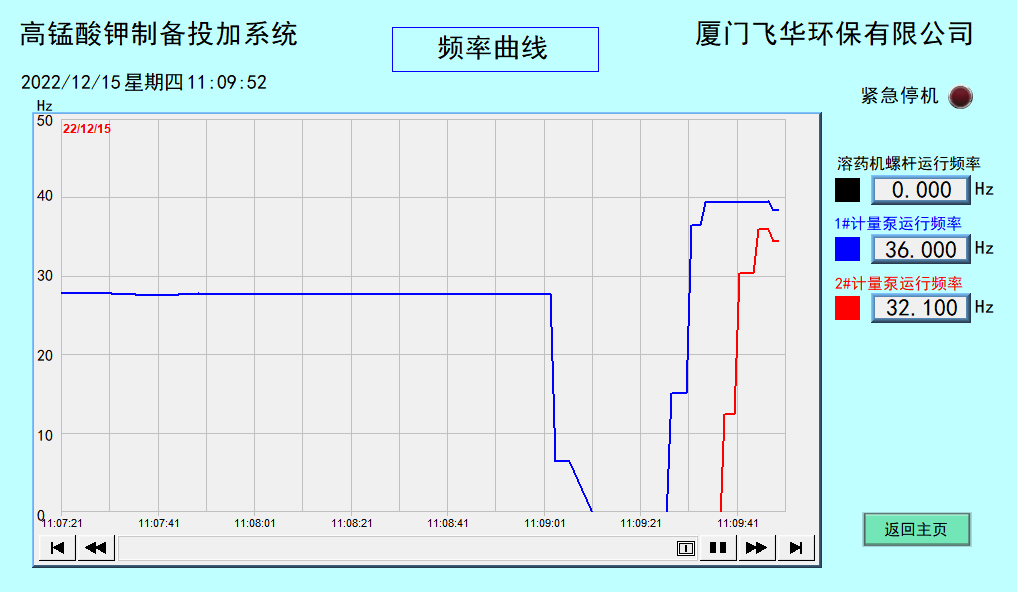
\includegraphics[height=5.5cm]{g10.PNG}};

                    %说明
                    \node at (-5,2) (2) [text_box] {料斗高料位探头};
                    \draw [arrow] (2) -- (0.5,2.2);
                    \draw (0.5,2.2) circle (0.5)[red];
                    \node at (-5,-1) (1) [text_box] {料斗低料位探头};
                    \draw [arrow] (1) -- (0.5,-0.2);
                    \draw (0.5,-0.2) circle (0.5)[red];

                    %辅助线
                    % \draw (-8,-2) [help lines] grid (8,2);
                    % \draw [red] (-8,0) -- (8,0);
                    % \draw [red] (0,-2) -- (0,2);
                \end{tikzpicture}
                \caption{料斗高低料位探头}\label{fig:g18}
            \end{figure}

            \par 料斗高低料位探头
            位置如上图\ref{fig:g18}所示。
            更换
            料斗高低料位探头
            之前,
            应先清理料斗内残留的高锰酸钾固体粉料。

            \newpage
        
        \subsubsection{搅拌机及螺旋进料器检修维护}
            检修维护搅拌机及螺旋进料器,
            特别是从装置上拆卸以及重新安装,
            有可能要打开制备系统的上盖,
            操作上较为复杂,
            建议联系加药系统经销商及售后服务人员处理。

            \begin{figure}[h]
                \centering
                \begin{tikzpicture}
                    %图片
                    \node  at (0,0) {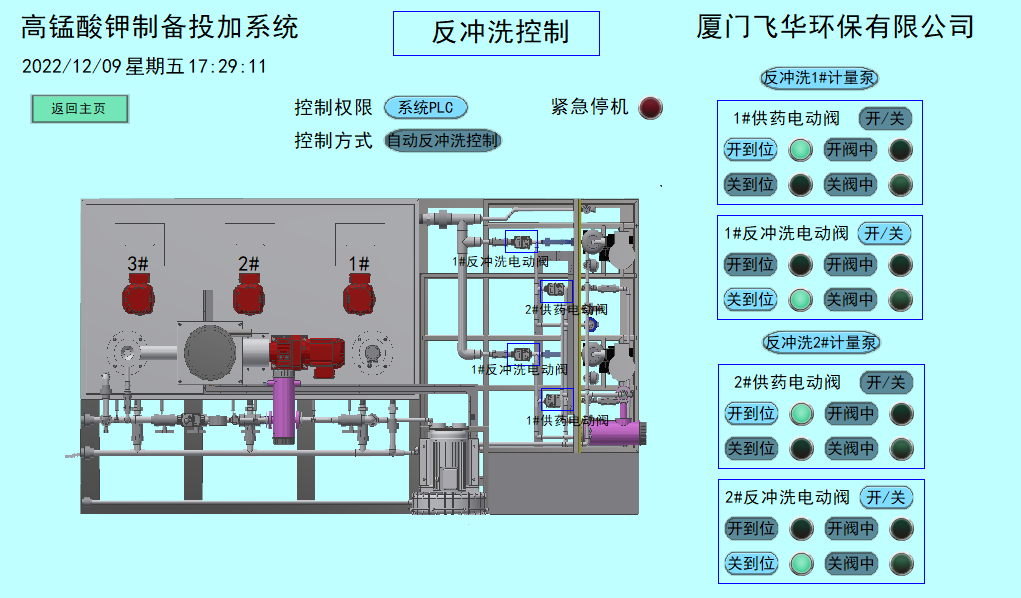
\includegraphics[height=10cm]{g3.PNG}};

                    %说明
                    \node at (4,-3) (2) [text_box] {排液阀};
                    \draw [arrow] (2) -- (1.2,-2);
                    \draw (1.2,-2) circle (0.5)[red];
                    \node at (3,-4) (1) [text_box] {排液阀};
                    \draw [arrow] (1) -- (-0.2,-2.8);
                    \draw (-0.2,-2.8) circle (0.5)[red];
                    \node at (2,-5) (3) [text_box] {排液阀};
                    \draw [arrow] (3) -- (-1.6,-3.5);
                    \draw (-1.6,-3.5) circle (0.5)[red];
                    \node at (-6,1) (4) [text_box] {连接活接};
                    \draw [arrow] (4) -- (-2.3,-0.8);
                    \draw (-2.3,-0.8) circle (0.5)[red];

                    %辅助线
                    % \draw (-8,-5) [help lines] grid (8,5);
                    % \draw [red] (-8,0) -- (8,0);
                    % \draw [red] (0,-5) -- (0,5);
                \end{tikzpicture}
                \caption{料斗高低料位探头}\label{fig:g19}
            \end{figure}

            \par 拆卸检修搅拌机及螺旋进料器之前,
            应先打开上图\ref{fig:g19}所示排液阀,
            排尽制备装置内液体,
            松开上图\ref{fig:g19}所示活接,
            才能打开制备系统上盖,
            检修或维护。

   \subsection{投加系统的检修维护}
        投加系统主要由
        计量泵、计量泵附件、流量探头、自动反冲洗系统组成。
        \par 上述设备均有2套各自独立,1用1备的系统,
        检修维护其中1套系统,
        不影响另外1套系统工作,
        满足高锰酸钾7*24小时投加的要求。
        \par 如果只是计量泵的阀球阀座之类卡了小型异物,
        可以只启动自动反冲洗系统,
        将小型异物冲走,
        不必拆卸维修。

        \subsubsection{关闭供药阀}
            检修前,
            应关闭检修工位的供药阀,
            防止储液槽内的高锰酸钾溶液,
            自流至检修工位范围内。
            \par 如果只是使用自动反冲洗系统,
            反冲洗管道,
            可跳过此步。

            \newpage
            
            \begin{figure}[h]
                \centering
                \begin{tikzpicture}
                    %图片
                    \node [rotate=-90] at (0,0) {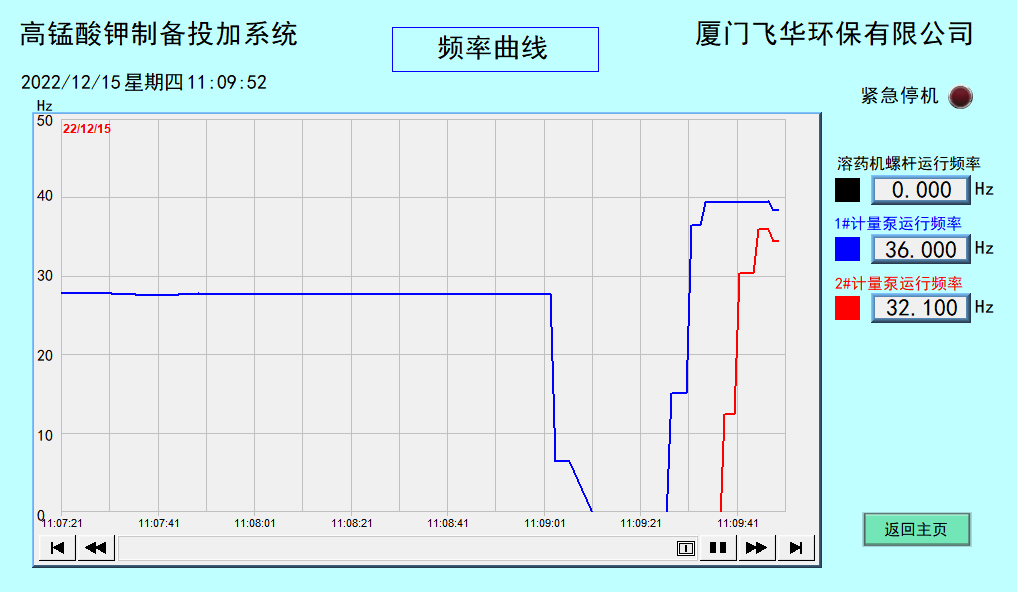
\includegraphics[height=9cm]{g10.PNG}};

                    %说明
                    \node at (-6,1) (1) [text_box] {供药阀};
                    \draw [arrow] (1) -- (-3.6,-0.8);
                    \draw (-3.6,-0.8) circle (0.5)[red];
                    \node at (-6,-4) (2) [text_box] {供药阀};
                    \draw [arrow] (2) -- (-2.5,-2.5);
                    \draw (-2.5,-2.5) circle (0.5)[red];

                    %辅助线
                    % \draw (-8,-5) [help lines] grid (8,5);
                    % \draw [red] (-8,0) -- (8,0);
                    % \draw [red] (0,-5) -- (0,5);
                \end{tikzpicture}
                \caption{供药阀位置}
            \end{figure}

        \subsubsection{反冲洗管道}
            投加系统配备自动反冲洗系统,
            进行检修维护之前,
            应启动自动反冲洗系统冲洗管道内化学品,
            再进行检修操作。
            \par  如果只是计量泵的阀球阀座之类卡了小型异物,
            可以只启动自动反冲洗系统,
            即可解决故障。
            \par 反冲洗过程完全自动,
            在人机界面上操作即可,
            操作过程如下图和图所示。

        \newpage

            \begin{figure}[h]
                \centering
                \begin{tikzpicture}
                    %图片
                    \node at (0,0) {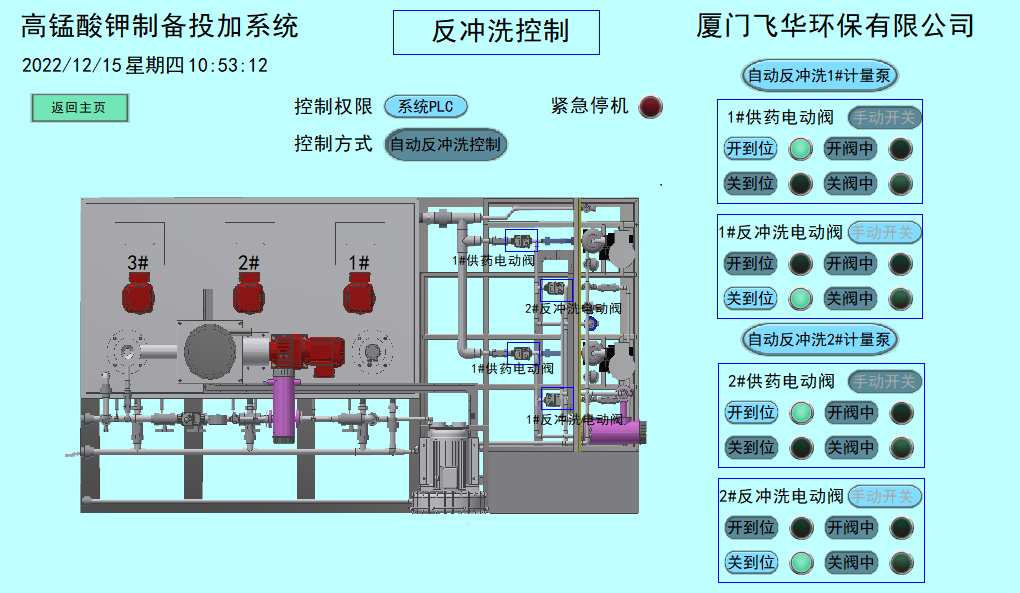
\includegraphics[height=8cm]{g6.PNG}};

                    %说明
                    \node at (-2,3) (1) [text_box, color=red] {自动反冲洗};
                    \draw (-3.5,2.1) rectangle +(1.5,0.6)[red];

                    %辅助线
                    % \draw (-8,-4) [help lines] grid (8,4);
                    % \draw [red] (-8,0) -- (8,0);
                    % \draw [red] (0,-4) -- (0,4);
                \end{tikzpicture}
                \caption{主控制界面}

                \vspace{6pt}

                \begin{tikzpicture}
                    %图片
                    \node at (0,0) {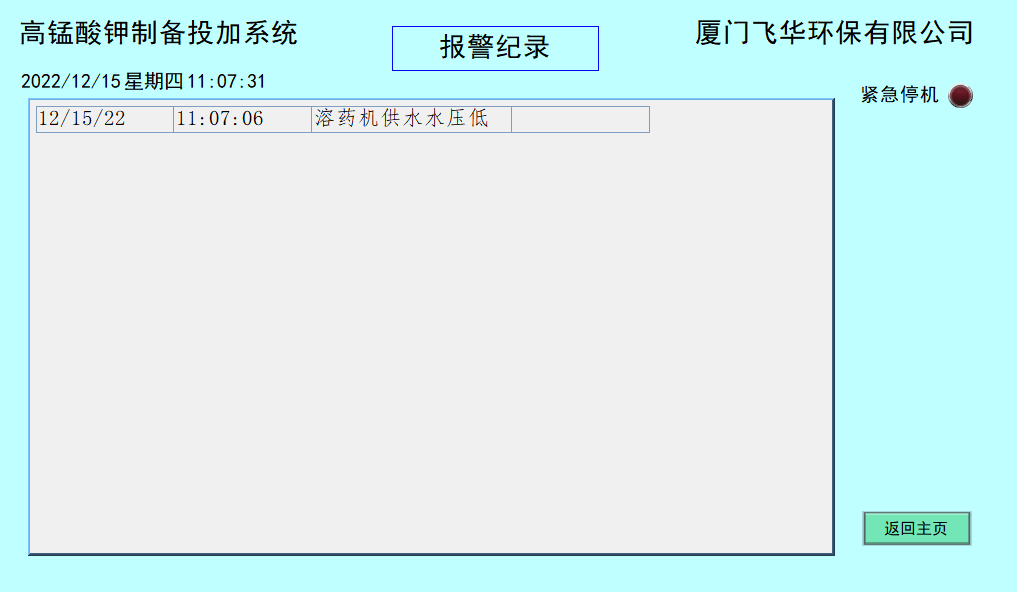
\includegraphics[height=8cm]{g8.PNG}};

                    %说明
                    \node at (6,3) (1) [text_box, color=red] {反冲1};
                    \node at (6,-0.6) (2) [text_box, color=red] {反冲2};
                    \draw (3.8,-0.9) rectangle +(1.8,0.5)[red];
                    \draw (3.8,2.6) rectangle +(1.8,0.5)[red];

                    %辅助线
                    % \draw (-8,-4) [help lines] grid (8,4);
                    % \draw [red] (-8,0) -- (8,0);
                    % \draw [red] (0,-4) -- (0,4);
                \end{tikzpicture}
                \caption{反冲洗控制按钮}
            \end{figure}

            \newpage

        \subsubsection{关闭相应工位的加药阀}
            检修前,
            应关闭检修工位的加药阀,
            防止下游管道内的化学品,
            回流至检修工位范围内。
            
            \begin{figure}[h]
                \centering
                \begin{tikzpicture}
                    %图片
                    \node [rotate=-90] at (0,0) {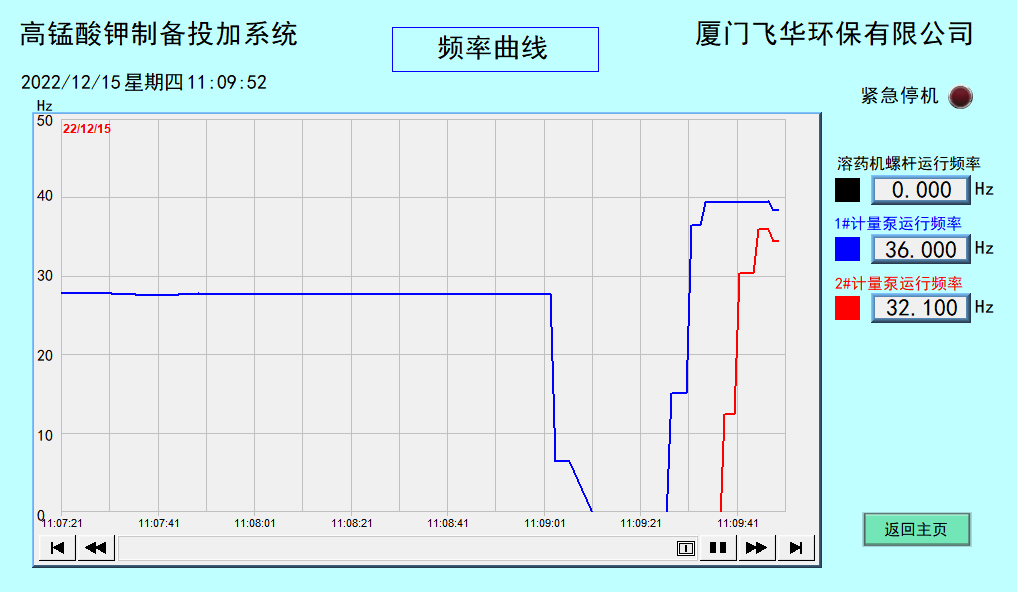
\includegraphics[height=9cm]{g10.PNG}};

                    %说明
                    \node at (-6,5) (1) [text_box] {加药阀};
                    \draw [arrow] (1) -- (-2,3.8);
                    \draw (-2,3.8) circle (0.5)[red];
                    \node at (6,5) (2) [text_box] {加药阀};
                    \draw [arrow] (2) -- (0.6,3.7);
                    \draw (0.6,3.7) circle (0.5)[red];
                    \node at (-6,-1) (3) [text_box] {排液阀};
                    \draw [arrow] (3) -- (-1.2,-0.2);
                    \draw (-1.2,-0.2) circle (0.5)[red];
                    \node at (6,-1) (4) [text_box] {排液阀};
                    \draw [arrow] (4) -- (1.2,-1.7);
                    \draw (1.2,-1.7) circle (0.5)[red];

                    %辅助线
                    % \draw (-8,-6) [help lines] grid (8,6);
                    % \draw [red] (-8,0) -- (8,0);
                    % \draw [red] (0,-6) -- (0,6);
                \end{tikzpicture}
                \caption{供药阀位置}\label{fig:g20}
            \end{figure}

        \subsubsection{打开相应工位的检修排液阀}
            \large{
                \textbf{
                    进行所有维护操作之前,
                    请先打开相应工位的检修排液阀,
                    释放系统内的压力!
                    否则,拆卸相关零部件时,
                    管道内的液体可能会喷射而出,
                    影响维修人员的安全!
                }
            }

            \par\normalsize{检修排液阀所在位置如上图\ref{fig:g20}所示。}

    \subsubsection{检修设备}
        待检修工位管道内残留化学品排净后,
        可对计量泵、阻尼器、隔膜压力表、背压阀、泄压阀、Y型过液器等设备或元件进行检修操作。
        \par 各设备或元件的检修方法,
        请参阅各设备或元件的使用说明,
        或咨询加药系统经销商或售后服务人员。

   \subsection{系统恢复运行}
        设备检修完成后,
        请关闭相应工位的检修排液阀,
        打开加药阀,
        打开供药阀,
        将投加系统的阀门都恢复至正常位置。
        \par 然后,
        请参阅第\ref{sec:sg1}章内容于第\pageref{sec:sg1}页,
        做好设备启动前准备,
        使系统处于待命状态,
        随时恢复正常运行。




\end{document}